In the traditional power system, the uncertainty in consumption causes imbalances. With the increase of wind energy and solar generation, the uncertainty traditionally only associated with consumption spreads to the production side. Furthermore, traditional sources of ancillary services are closing down, which means that TSOs must find new ways of balancing the system. Also, new problems will appear at the distribution system level, such as power congestion and voltage issues. These problems arise because of new consumption technologies appearing in the system, such as \glspl{ev} and \glspl{hp}, and because of new generation units, \eg \glspl{wt}, small size \glspl{chp} and \glspl{pv}, are installed at distribution level. All these new units in the electric power system are commonly referred to as \glspl{der}\footnote{In this work the concept of DER includes \gls{dg}, \gls{ee}, demand response (DR) and \gls{dess}, which is a combination of the the traditional definition of DER = DG + DESS (as seen in \eg \cite{nrel2002using}) and the broader definition presented in \cite{nys2014reforming}.} or flexible resources. It is the responsibility of the \gls{dso} to resolve the problems arising due to the integration of the DERs, which can be the overloading of system components or voltage issues. These problems affect the quality of the power supply at residential level, but can also lead to issues at transmission level.
\begin{figure}[ht]
	\centering
	\caption{The Electric Power System of tomorrow contains a large ICT infrastructure, which permits the flow of information and control between the system actors. Furthermore, the flow of electricity is not only from generator to consumer, but there is also intermittent electricity generation at distribution level.}
	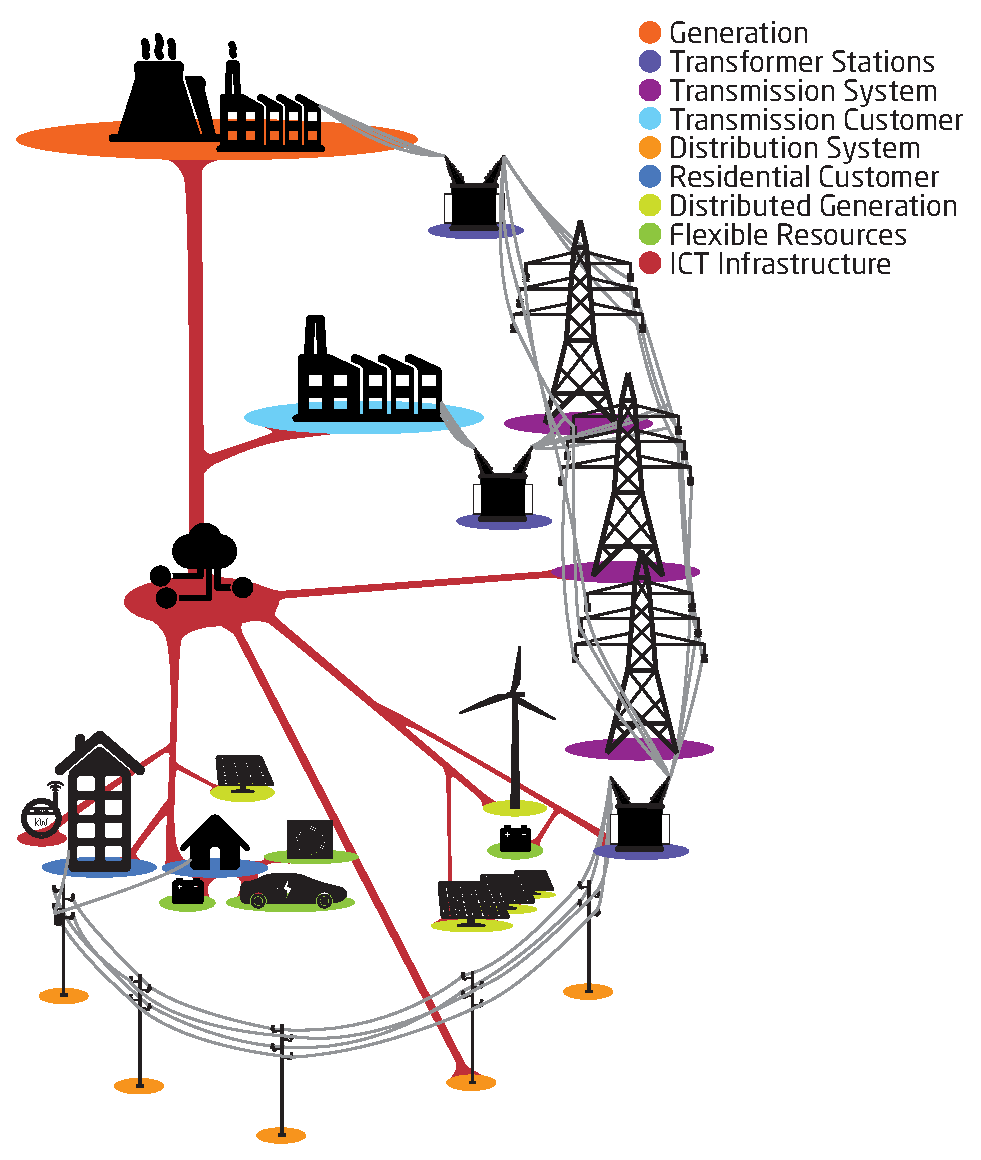
\includegraphics[width=\textwidth]{intro/smart_grid_new.eps}\label{fig:powerfuture}
\end{figure}

The expected future smart grid can be seen in Figure~\ref{fig:powerfuture}, where not only the new DERs appear but an \Gls{ict} infrastructure coordinates the behaviour of the units for the benefit of the system. Smart metering is added at consumer level, and sensors are deployed at distribution level.
\begin{figure*}[htbp!]
	\centering
	\caption{The actors and relationships in the power market of tomorrow. Compared to the current market setup, the aggregator entity has been added, as well as the ability of DSOs to contract ancillary services. Also, the consumer becomes a player in the electricity markets through the aggregator.}
	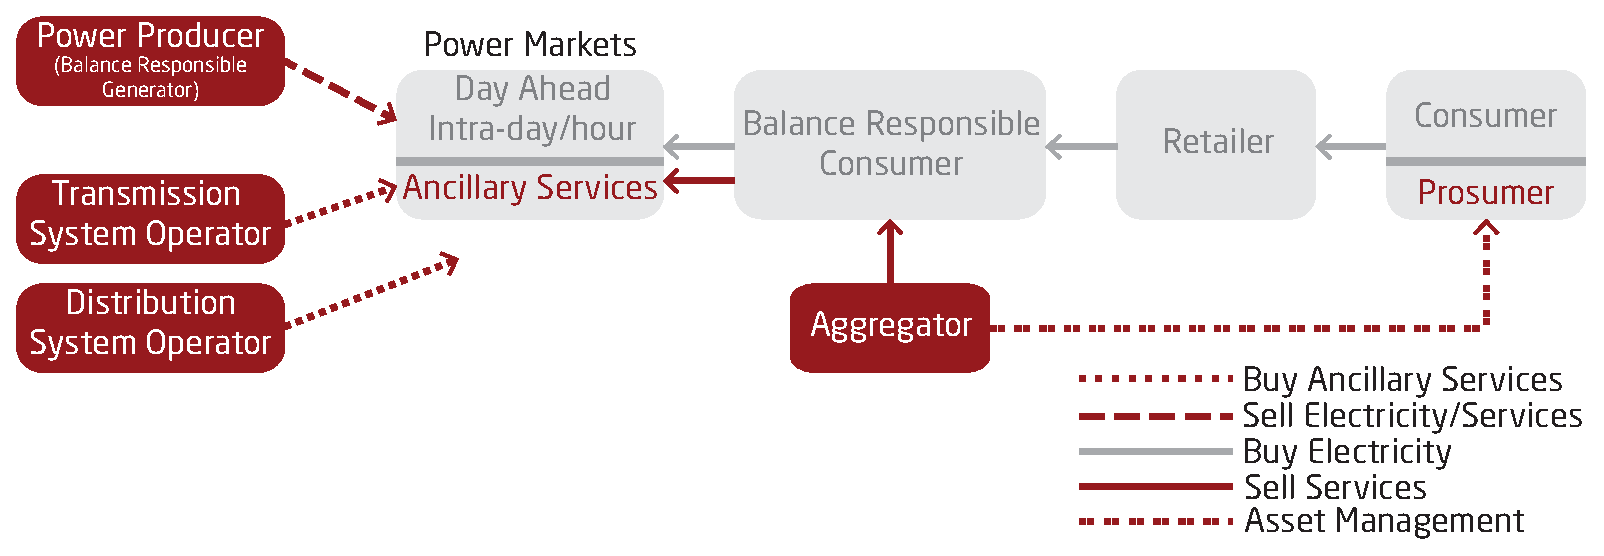
\includegraphics[width=\textwidth]{intro/market_future.eps}\label{fig:marketfuture}
\end{figure*}

In order to cope with the new problems, both at transmission and distribution level, it is expected that consumers will become prosumers. That is, the consumers will take an active role in the power markets by selling services to the system operators through an aggregator\footnote{The concept of the aggregator is further discussed in Chapter~\ref{cha:aggregator}.}. The aggregator will provide an asset management service to the end consumer, and by managing a pool of consumers, it will be able to control a large enough consumption volume to provide ancillary services to the system operators, or balancing services to the consumption BRP. The action of a consumer changing his or her consumption based upon an incentive is known as \gls{dr}. The aggregator facilitates DR by providing the ICT infrastructure and control infrastructure to DER owners, as well as statistical certainty of service delivery and legal responsibility towards the system operators. The aggregator can be an independent commercial entity, or it can be a function inside one of the pre-existing market players. The new market setup can be seen in Figure~\ref{fig:marketfuture}, and it shows how the aggregator entity will interact with the existing market setup, and how the DSO will become a new player in the market, which will acquire services to resolve some of it problems.

In conclusion, we see the electric power system moving away from a \emph{production-must-follow-consumption} pattern to \emph{consumption-should-partly-follow-production} and hereby facilitate the integration of renewables and DERs. An integral part of achieving this change will be the use of control services to change the consumption behavior of units in the network. Given that the units providing ancillary services to the grid are critical for the security of the system, the new control algorithms and infrastructure must be validated.


